\chapter{MLops}
Una tipica pipeline per un progetto di machine learning è composta da diverse fasi:
\begin{itemize}
      \item Comprensione del problema
      \item Raccolta dei dati
      \item Comprensione dei dati
      \item Preparazione dei dati
      \item Modellazione
      \item Valutazione
      \item Deployment
\end{itemize}
\begin{figure}[!ht]
      \centering
      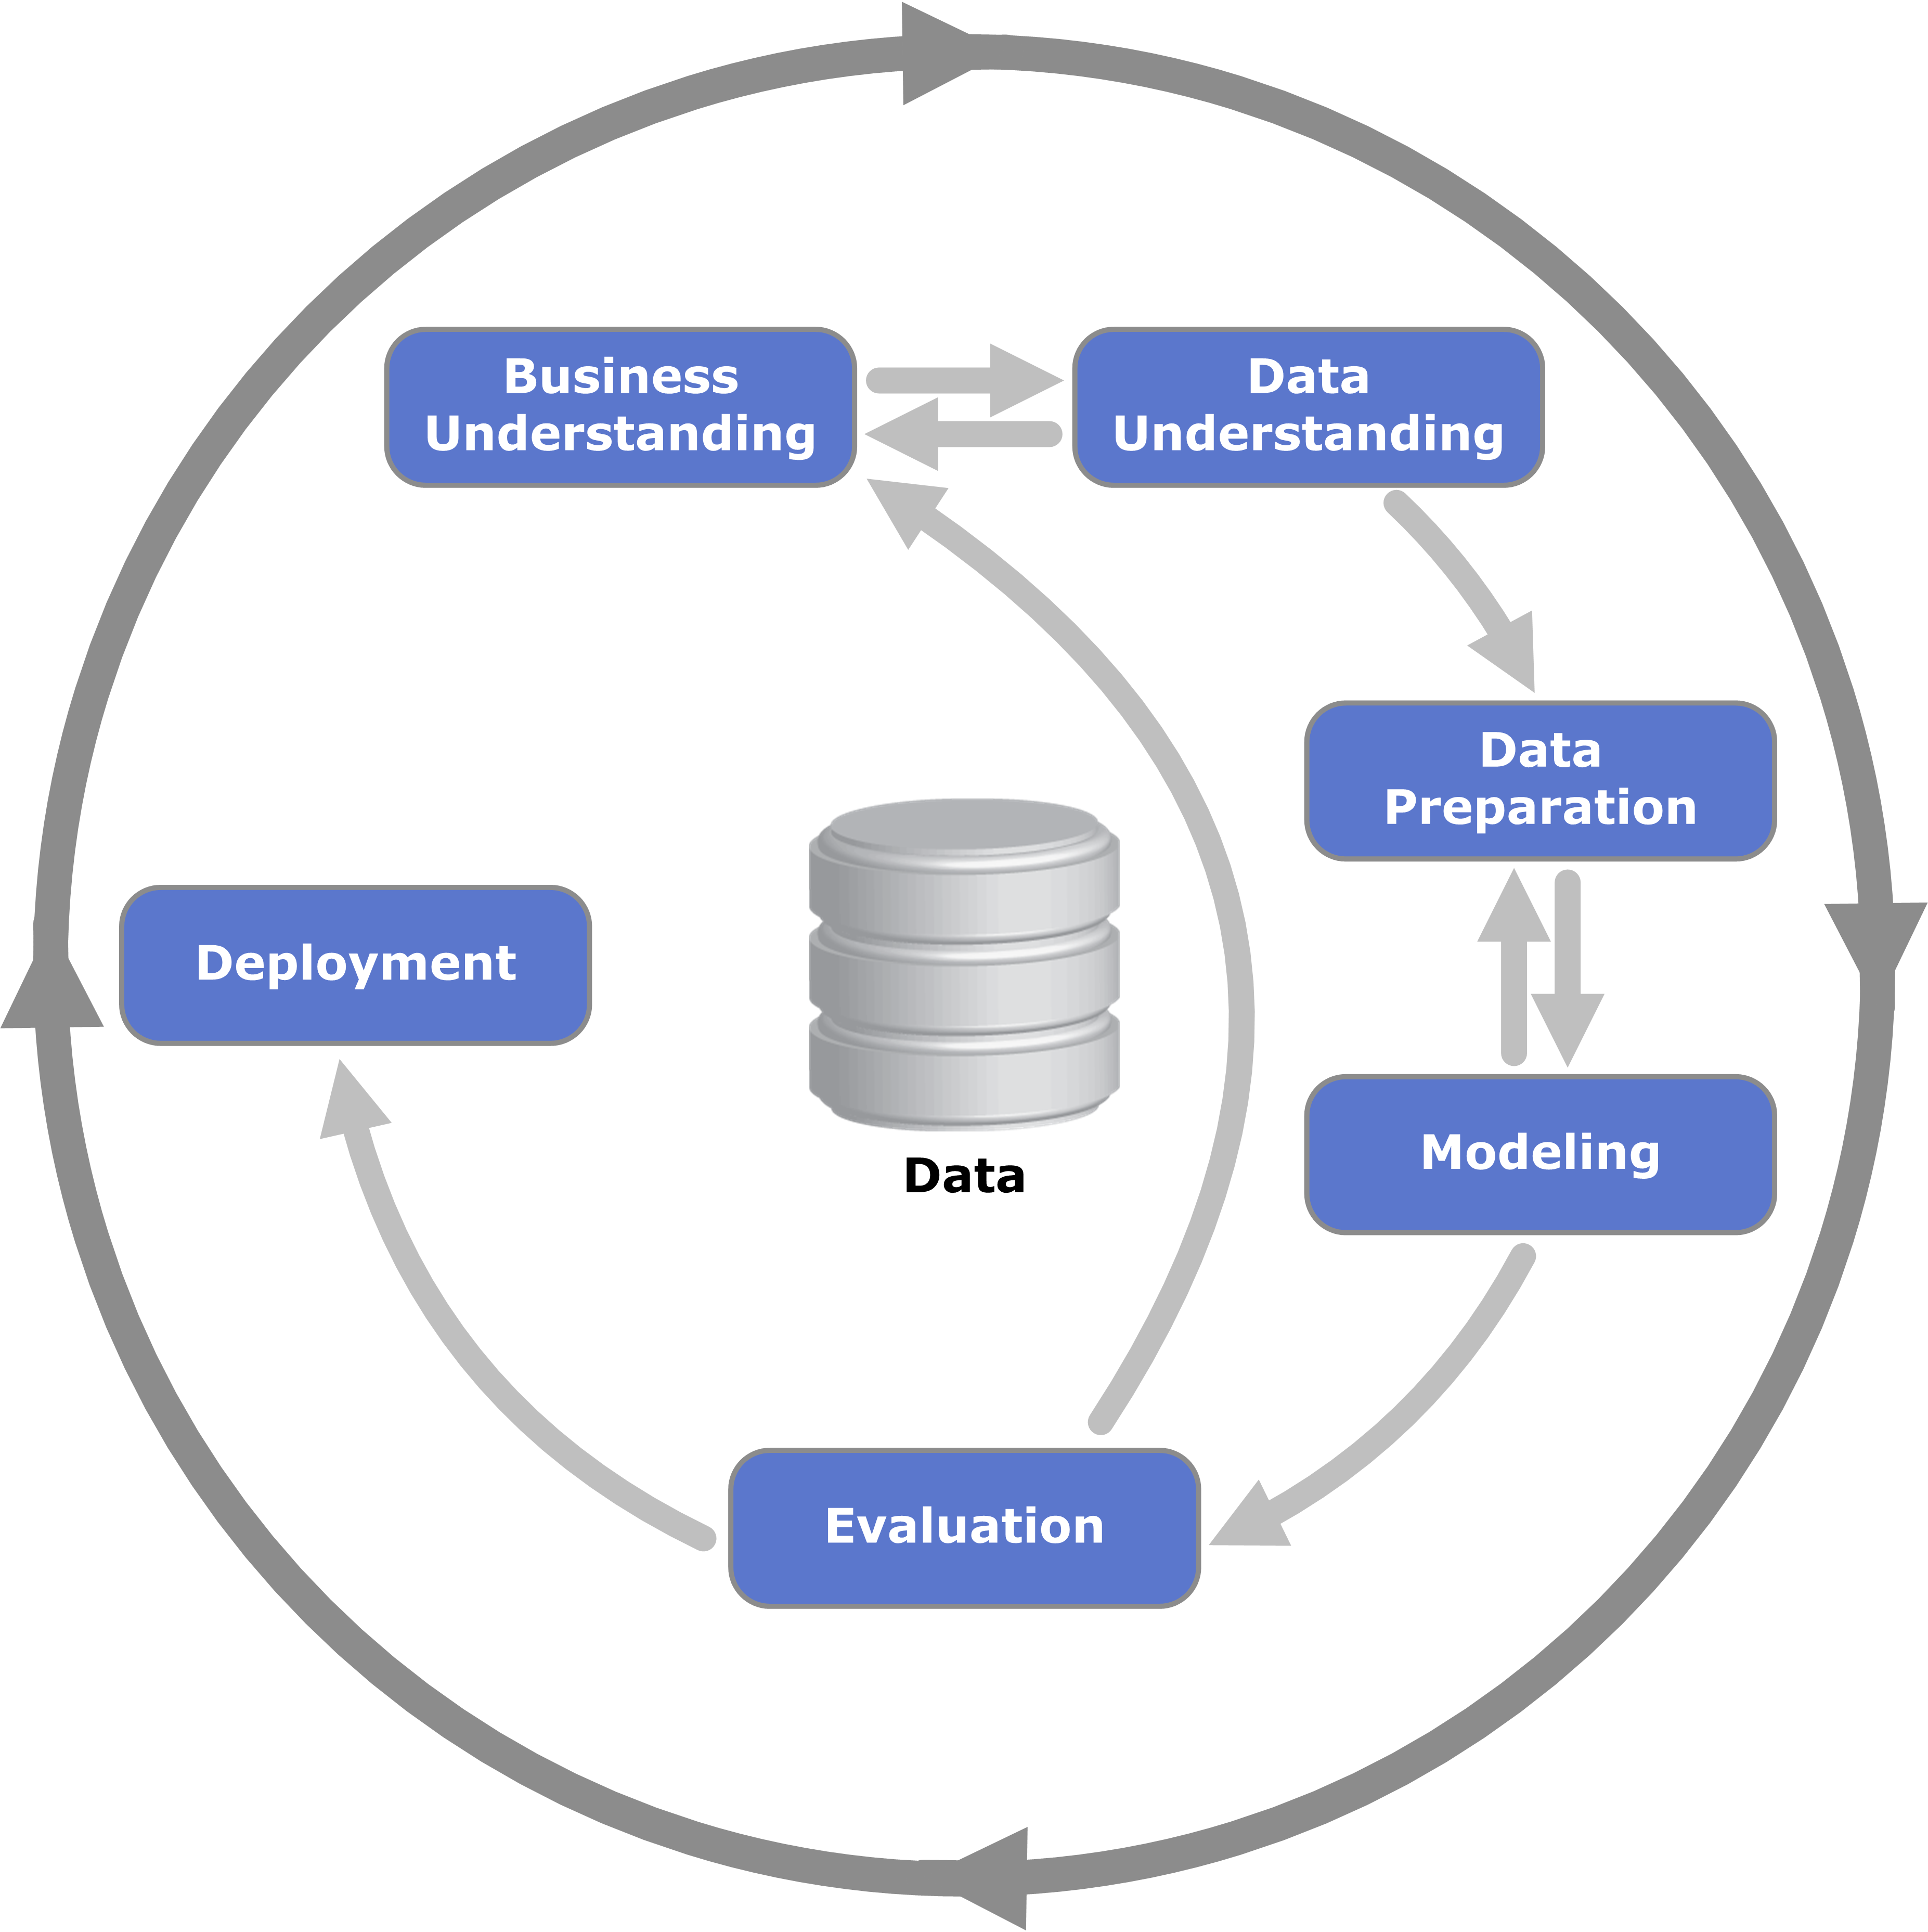
\includegraphics[width=0.5\textwidth]{./img/MLops/CRISP-DM.png}
      \caption{ML Pipeline}
      \label{fig:ml_pipeline}
\end{figure}
In questa parte del corso ci occuperemo della parte di gestione dei dati, nello
specifico analizzeremo la parte di \textbf{Data Understanding} e \textbf{Data
      Preparation}.

Avere i dati corretti è una parte fondamentale per la creazione di un modello di
che sia in grado di ottenere dei risultati corretti.
\begin{center}
      \textit{Garbage in, garbage out}
\end{center}
I dati di training e testing devono derivare dai dati reali che verranno raccolti
in fase di production.
\section{Pipeline}
Una volta ottenuti i dati reali dovremo separarli in:
\begin{itemize}
      \item \textbf{Training data}: vengono utilizzati per addestrare e valutare
            il modello, sono quindi di dimensioni elevate e vengono raccolti
            attraverso diverse fonti. Spesso caratterizzati da un elevato throughput.
      \item \textbf{Serving data}: raccolti e utilizzati per fare previsioni in
            fase di production. Questa tipologia di dati è spesso caratterizzata
            da una bassa latenza.
\end{itemize}
Entrambi questi tipi di dati devono passare attraverso una fase di \textbf{preparazione}.
In questa fase si vogliono stabilire quali sono le informazioni principali,
quali dati sono rilevanti e quali dati sono irrilevanti. Si effettua dunque una
prima analisi. Inoltre, vengono eseguite diverse operazioni per far si che i dati
si adattino al modello che si vuole creare.

Prima di arrivare alla parte di addestramento del modello, si passa attraverso una
fase di \textbf{validazione dei dati}. Questa fase è necessaria in quanto i dati cambiano
o cambia il contesto.
L'obiettivo principale è quello di capire quali feature sono significative
per il modello e quali no. Questo serve per controllare in futuro se queste
feature significative sono cambiate.
Questa fase viene fatta confrontando le distribuzioni delle features ritenute
significative durante il training con la distribuzione delle stesse feature prese
dai dati raccolti in produzione.
In questo modo possiamo segnalare quando le distribuzioni cambiano e nel caso devo
adottare delle soluzioni:
\begin{itemize}
      \item Riaddestrare il modello.
      \item Avvisare l'utente che qualcosa sta cambiando.
      \item Non fare niente.
\end{itemize}
Può capitare nel tempo i le feature cambino il tipo (ad esempio si passa da int
a float), quindi, nella fase di validation, bisogna correggerli per renderli
compatibili col modello.

Per effettuare tutti i passi della pipeline servono diverse figure lavorative:
\begin{itemize}
      \item \textbf{Machine Learning Expert}
      \item \textbf{Software Engineer}
      \item \textbf{Site Reliability Engineer}: esperto che si occupa di gestire
            tutta la pipeline e di risolvere eventuali problemi.
\end{itemize}

Nella fase di preparazione dei dati si possono avere diverse fasi che permettono
la corretta gestione e formulazione del dataset da utilizzare per il modello di ML.
\section{Data Acquisition}
Una delle fasi più importanti è \textbf{Data Acquisition} che si articola nell'acquisizione
dei dati per la creazione del dataset, spesso si utilizzano diverse fonti.
In questa fase possiamo
avere diversi problemi nell'acquisizione dei dati
come ad esempio l'introduzione di bias che invalidano i risultati del modello.
I bias possono essere di due tipi:
\begin{itemize}
      \item storici: ex: se si vuole predire il futuro presidente degli USA,
            se si allenasse l'algoritmo con dati storici sicuramente non potrà predire
            una donna.
      \item rappresentativi: ex: se si vuole sviluppare un riconoscimento facciale
            allora non possiamo allenarlo solo su individui di un continente.
\end{itemize}

In aggiunta, quando si deve creare un dataset è obbligatorio sapere la
\textbf{Data Provenance} ovvero documentare
come ho costruito il dataset di training e validation. Questo consiste nel sapere
quali sono i dati utilizzati, da dove vengono, come ho costruito il dataset. In
questo modo si risolvono eventuali problemi dovuti a risultati sballati per dati
che sono stati iniettati nel dataset.
\section{Data Understanding}
Una volta acquisiti i dati, il primo passo consiste nella loro comprensione,
quindi di passa per una fase di \textbf{data exploration}.
Questa fase viene fatta dopo aver creato il dataset e prima di effettuare il training
o il serving dei dati, in modo da capire se i dati sono consistenti e se sono stati raccolti in modo
corretto, generalmente si implementa con dei \textbf{sanity checks}.

I dati che vengono raccolti sono solitamente rappresentati sotto forma tabellare,
e possono essere:
\begin{itemize}
      \item \textbf{Discreti}: valori che possono essere rappresentati da un insieme
            finito o numerabile di valori. Possiamo inoltre avere anche due sotto
            categorie:
            \begin{itemize}
                  \item \textbf{Categorici}: valori che rappresentano delle categorie.
                  \item \textbf{Count}: valori che rappresentano il numero di
                        occorrenze di un certo evento.
            \end{itemize}
      \item \textbf{Continui}: valori che possono essere rappresentati da un insieme
            non numerabile di valori.
\end{itemize}
L'esplorazione dei dati avviene attraverso dei \textbf{sanity checks}, ovvero dei
controlli che vengono svolti per studiare l'integrità dei dati. Un esempio di sanity
check può essere il controllo della latitudine e longitudine di un punto, questi
valori devono essere compresi in un certo range.

Un ulteriore controllo viene fatto sul bilanciamento delle features, in particolare,
per quelle categoriche si controlla se la distribuzione degli esempi per ogni
categoria è bilanciata. In caso contrario, la feature potrebbe non essere significativa
oppure si potrebbe avere un bias nei dati.

Un altro controllo che viene fatto è il controllo della cardinalità delle features.
Ad esempio, una persona non può avere associata più di una data di nascita.

Tutti questi controlli possono essere essere effettuati attraverso diverse modalità:
\begin{itemize}
      \item \textbf{Visualizzazione}: attraverso grafici e tabelle.
      \item \textbf{Query SQL}: attraverso query che permettono di estrarre
            informazioni dai dati.
      \item \textbf{Script}: attraverso script che permettono di estrarre
            informazioni dai dati.
\end{itemize}

Per gestire le inconsistenze scoperte dai sanity checks si possono adottare diverse
strategie:
\begin{itemize}
      \item Eliminare l'esempio, questa strategia può essere adottata solamente
            nel caso in cui il numero di esempi eliminati non sia troppo elevato.
      \item Correggere l'errore con metodi di imputazione, bisogna però stare
            attenti perché non sempre si può fare. Per esempio, se i dati
            rappresentati da una feature sono vincolati da qualche normativa,
            non posso correggere l'errore con un metodo di imputazione.
\end{itemize}

Riassumendo, la fase di data exploration è composta dai seguenti passi:
\begin{itemize}
      \item \textbf{Identificazione delle variabili}: quali sono le variabili che ho
            a disposizione e che ruolo hanno.
      \item \textbf{Analisi univariata}: analisi delle variabili una alla volta.
            Voglio capire se la variabile in analisi è continua o discreta,
            studiare la sua distribuzione e capire se ci sono degli outlier. Questo
            può essere fatto attraverso l'utilizzo di box plot e istogrammi.
      \item \textbf{Analisi bivariata}: analisi tra coppie di variabili. Voglio
            capire come le variabili interagiscono tra di loro. Questo può essere
            fatto attraverso l'utilizzo di scatter plot.
      \item Capire se ci sono valori mancanti e come gestirli.
      \item identificare e gestire i valori anomali (outlier).
\end{itemize}

\begin{definizione}
      L'\textbf{Exploratory Data Analysis} (EDA) è una tecnica statistica che permette
      di esplorare i dati e di estrarre informazioni utili per la costruzione di un
      modello.
\end{definizione}

Tra le varie tecniche di analisi dei dati abbiamo:
\begin{itemize}
      \item \textbf{Measure of dispersion}: permette di capire la dispersione
            dei dati, vovero quanto i dati sono
            distanti tra di loro. Questo può essere fatto attraverso l'utilizzo
            di varianza, deviazione standard, media, quantili e altre misure statistiche.
      \item \textbf{Box plot}: permette di visualizzare la distribuzione dei dati
            attraverso quartili.
      \item \textbf{QQ plot}: permette di confrontare la distribuzione dei dati
            con una distribuzione normale.
      \item \textbf{Scatter plot}: permette di visualizzare la relazione tra due
            variabili evidenziando eventuali correlazioni.
      \item \textbf{Swarm plot}: permette di visualizzare la distribuzione dei dati
            in base ai valori che può assumere la variabile categorica.
\end{itemize}

\begin{figure}[!h]
      \centering
      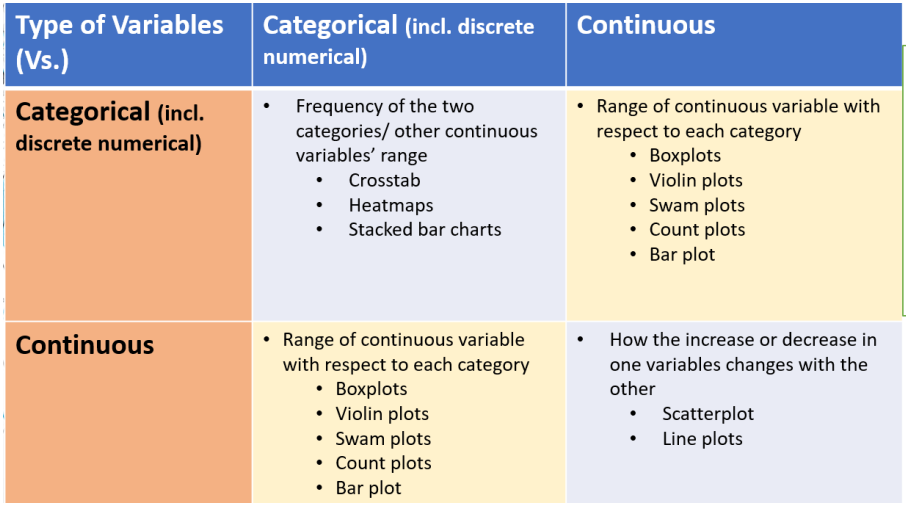
\includegraphics[width=0.7\textwidth]{img/MLops/exploration.png}
\end{figure}

Le visualizzazioni sono spesso guidate dai dati quindi varieranno in base alle
caratteristiche degli attributi.

Queste analisi sono fondamentali per capire se i dati sono soggetti a dei bias,
quindi risulta importante effettuare tutte queste analisi durante tutto il data lifecycle,
questo perché mi aiuta ad individuare eventuali problemi e a correggerli.

Le metodologie descritte in questo capitolo non rappresentano un processo che deve
essere seguito alla lettera, ma sono delle linee guida che possono essere adattate
in base al contesto. Ogni dominio applicativo richiede delle analisi specifiche.
In aggiunta, quando addestriamo un modello di machine learning dobbiamo capire se
il suo comportamento è \textbf{fair}, ovvero se il modello non è influenzato da
bias.
\section{Data validation}
Nella fase di sviluppo e mantenimento di un modello dobbiamo sempre controllare
che la distribuzione dei dati non sia cambiata durante il tempo.
Ovvero, che i valori su cui vogliamo effettuare delle previsioni abbiano la stessa
struttura dei dati di training.

Questa analisi è molto importante perché se si modifica un dato allora dobbiamo
accorgercene e modificare il modello di conseguenza.

Un esempio di cambiamento può essere il seguente:
\begin{itemize}
      \item Abbiamo una feature di tipo string che passa da Upper case a lower case.
      \item Le variabili che cambiano di semantica. Ad esempio il numero di giorni
            che diventa numero di ore.
      \item Scompare un attributo, diventa null.
\end{itemize}
Risulta quindi fondamentale avere un sistema di riconoscimento delle anomalie
nei dati. Questo sistema deve essere in grado di riconoscere quando i dati cambiano
e deve essere in grado di produrre un \textbf{alert}.

Solitamente, in relazione con gli alert si costruisce un \textbf{playbook} che
specifica chi deve essere avvisato e come risolvere il problema.

In questo modo, quando si riceve un alert si sa già come risolverlo, seguendo
le specifiche descritte nel playbook.
\section{Data Integration}
Con il termine \textbf{data integration} si intende la fase in cui si uniscono
diverse sorgenti di dati in un'unica sorgente. La complessità di questa
fase si palesa quando le sorgenti dati presentano una grande sovrapposizione tra
di loro. Posso risolverlo in primo luogo utilizzando delle \textbf{join}.

Per effettuare questa operazione bisogna per prima cosa identificare lo schema
delle sorgenti che si vogliono unire. Fatto ciò, bisogna trovare gli attributi
che sono in comune tra le sorgenti in modo da poterli utilizzare per effettuare
il join.

Questa fase può essere più complicata perché potremmo dover effettuare l'integrazioni
tra modelli di dati differenti. Non solo, potremmo avere delle eterogeneità a livello
di nomi e anche di tipo, un esempio è il sistema di valutazione universitario
che può essere espresso in modi diversi: $0-30$, $A-F$. Possiamo avere problemi
come rappresentazioni di entità in una sorgente mentre nell'altra può essere
modellata come attributo.

Un generico modo per risolvere questi problemi:
\begin{itemize}
      \item \textbf{Definizione dello schema finale}: si definiscono anche le regole di
            mappatura degli schemi delle sorgenti nello schema finale.
      \item \textbf{Schema matching}: si definiscono delle regole di investigazione su come
            effettuare il matching. In questa fase si vuole capire se ci si basa
            solo sul nome dell'attributo oppure anche sul valore di esso. Inoltre,
            si specificano regole di investigazione.
      \item \textbf{Schema integration}: si effettua direttamente l'integrazione dei dati.
\end{itemize}
Vediamo ora nello specifico il processo di integrazione, analizzando cosa ogni
fase comporta:
\begin{enumerate}
      \item \textbf{Schema Integration}: in questa fase si prendono in input $n$
            schemi di partenza e si vogliono omogeneizzare in modo da poter fare
            il join. Per questa fase solitamente si utilizzando metodi di \textbf{
                  model transformation} e \textbf{reverse engineering}.
      \item \textbf{Correspondences Investigation}: in questa fase si vogliono
            capire le corrispondenze tra gli schemi. Questo può essere fatto
            attraverso l'utilizzo di tecniche per la scoperta di corrispondenze.
            In output si ottengono le corrispondenze tra gli schemi.
      \item \textbf{Schema integration and mapping}: in questa fase si vogliono
            integrare gli schemi e mapparli in modo da poter fare il join. Per
            fare questo si utilizzano le informazioni recuperate nella fase
            precedente. In output si ottiene lo schema integrato.
\end{enumerate}

Le metodologie per effettuare le integrazioni sono differenti, per esempio possiamo
avere due metodi:
\begin{itemize}
      \item \textbf{Binario}: si considerano le sorgenti due a due ricorsivamente.
      \item \textbf{n-ario}: si uniscono più scorgenti alla volta.
\end{itemize}

\begin{figure}[!ht]
      \centering
      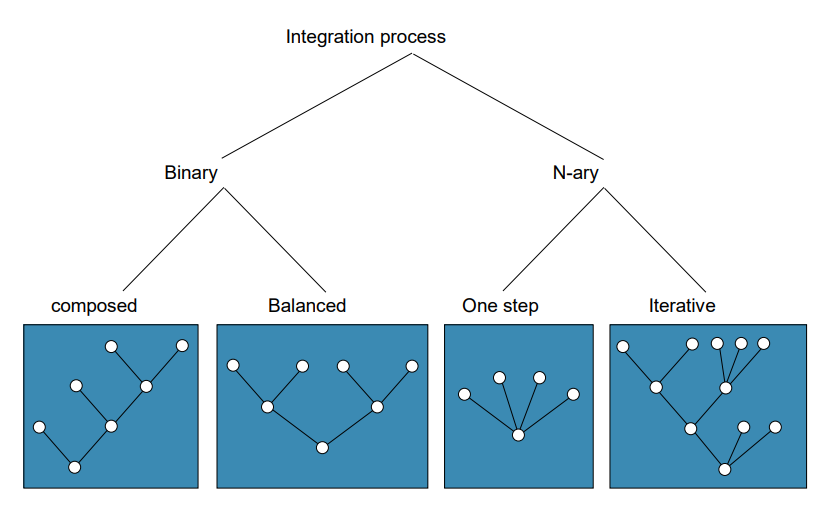
\includegraphics[width=0.5\textwidth]{./img/MLops/data_integration.png}
      \caption{Data Integration}
      \label{fig:data_integration}
\end{figure}
Uno primo problema che si può avere durante l'integrazione sono i \textbf{conflitti descrittivi}
dove differenti proprietà vengono descritte in modi differenti:
\begin{itemize}
      \item \textbf{conflitti di nomi}: spesso sono conflitti che appaiono nei nomi
            di oggetti, entità e relazioni. Questi conflitti possono essere di \textbf{sinonimi}
            (ex: usiamo da una parte nodo e dall'altra estremità), oppure possono essere
            di \textbf{omonimi} (ex: usiamo da una parte Highway (EU) e dall'altra Highway (USA))
      \item \textbf{conflitti di composizione}: da una sorgente abbiamo gli Utenti
            specificati con degli alttributi, mentre in un altra sorgente abbiamo gli
            Utenti specificati in un altro modo.
\end{itemize}

Un altro problema è sono i \textbf{conflitti di frammentazione}, stesse istanze
rappresentante in due sorgenti diverse che possono avere valori degli attributi
differenti:
\begin{itemize}
      \item \textbf{Conflitto di chiave}: due record uguali che hanno chiavi
            differenti. Per risolvere questi problemi o sfruttiamo le conoscenze
            del dominio.
      \item \textbf{Conflitto di attributi}: devo decidere a priori se considerare
            il valore di una tabella o l'altra in base alla conoscenza del dominio,
            perché magari è più corretto rispetto all'altra.
\end{itemize}

\begin{nota}
      Nessuna metodologia è sbagliata, l'importante è documentare le scelte fatte
      e restare coerenti.
\end{nota}

Le tecniche per risolvere i conflitti a livello di istanza si differenziano in
\textbf{design time} e \textbf{run time}. In entrambi i casi il conflitto si
verifica a \textit{query time}, ma a design time si sceglie la politica mentre a
run time si esegue. In entrambi i casi, possiamo usare delle funzioni di
risoluzione dei conflitti (COUNT, MIN, MAX\dots).

Una volta integrate le sorgenti, dobbiamo occuparci della rimozione dei \textbf{duplicati}.
Per farlo, la prima operazione consiste nel \textbf{riconoscerli}, questo perché ci possono
essere valori duplicati che non sono subito riconoscibili a causa di errori,
ex: concettualemente due record rappresentano la stessa istanza ma non si riconoscono
perché hanno attributi con errori che rendono sintatticamente differenti i due record.
Per svolgere questa operazione, spesso si sfrutta la conoscenza del dominio.
Può capitare che la fase di rimozione dei duplicati porti alla necessità di
fondere due righe. Questo perché potremmo avere due righe che rappresentano la
stessa entità ma che hanno valori diversi. In questo caso, si fondono le righe
in modo da ottenere una sola riga contenete i valori corretti.
Per confrontare le righe e riconoscere se sono dei duplicati ci possono essere diversi metodi:
\begin{itemize}
      \item \textbf{Empirical}: si confrontano i valori delle righe e si decide
            se sono uguali o meno in base a delle regole. Per le stringhe ad
            esempio, si possono confrontare le lettere che le compongono.
      \item \textbf{Probabilistici}: si normalizzano i formati degli attributi,
            ovvero si portano a un formato standard, a questo punto si suddividono
            i record in blocchi e si confrontano, questo mi permette di ordinare
            il blocco per qualche attributo molto discriminante. Il confronto viene
            fatto mediante delle funzioni, spesso si confrontano i più vicini
            nella realtà.
      \item \textbf{Knowledge-based}: si utilizza la conoscenza del dominio per
            confrontare i record.
      \item \textbf{Machine Learning}: si utilizzano modelli di machine learning
            per confrontare i record.
      \item \textbf{Mixed}: si utilizzando metodi Probabilistici e Knowledge-based
            insieme.
\end{itemize}
\section{Data Enrichment}
Il \textbf{data enrichment} è una fase in cui si vogliono arricchire i dati con
nuove informazioni presenti in altre sorgenti. Nel fase di data integration
avremo che una riga può essere associata con una sola riga nella seconda sorgente.
In questo caso possono avere che una riga è associata con più righe della seconda
tabella.
\section{Feature engineering}
Il \textbf{feature engineering} è un insieme di operazioni per aggiungere nuove
feature o rimuovere righe, modificarle etc.

Queste operazioni si dividono in:
\begin{itemize}
      \item \textbf{Target transformation}: trasformiamo un'etichetta da $0-1$ a
            etichetta o viceversa. In base a come cambiamo il target otteniamo
            risultati differenti.
      \item \textbf{Feature enconding}: trasformare un attributo in più attributi.
            Questo viene spesso usato per i categorici, ad esempio one hot encoding.
      \item \textbf{Feature extraction}: estrazione di feature dai dati raw.
            Molto spesso nella realtà abbiamo dei dati raw che devono essere
            etichettati. Questa operazione risulta molto costosa perché richiede
            esperti del dominio. Inoltre, effettuare un'etichettatura superficiale
            porta a delle performance peggiori del modello.
      \item \textbf{Feature selection}: si selezionano le feature del dataset
            che sono le più rilevanti, esistono approcci matematici come PCA e RP.
            Oltre a questi metodi, possiamo utilizzare anche metodi supervisionati,
            i quali addestrano modelli per effettuare la selezione delle feature.
            Oppure, possiamo utilizzare anche algoritmi non supervisionati.
            \begin{figure}[!ht]
                  \centering
                  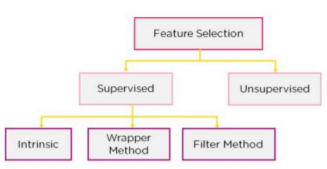
\includegraphics[width=0.5\textwidth]{./img/MLops/feature_selection.png}
                  \caption{Feature Selection}
                  \label{fig:feature_selection}
            \end{figure}
\end{itemize}
\subsection{AutoML}
Con il termine \textbf{AutoML} si indicano delle tecniche che permettono di
automatizzare la pipeline di un progetto di machine learning. Nello specifico,
queste tecniche permettono di automatizzare la fase di feature engineering,
creazione del modello e valutazione di esso. Questo permette di ridurre il lavoro
che svolge il data scientist, il quale si occupa solo della raccolta dei dati raw
e prepararli per passarli al processo di AutoML.

L'implementazioni di questi metodi viene fatta sfruttando la conoscenza e
l'esperienza sviluppata nel corso degli anni.
\section{MLops}
Come per lo sviluppo del software, il quale è in continua evoluzione, anche lo
sviluppo di una pipeline di machine learning cambia nel tempo. Per questo motivo
è stato introdotto il concetto di \textbf{MLops}, il quale estende il concetto di
DevOps includendo la parte di machine learning.
\begin{figure}[!ht]
      \centering
      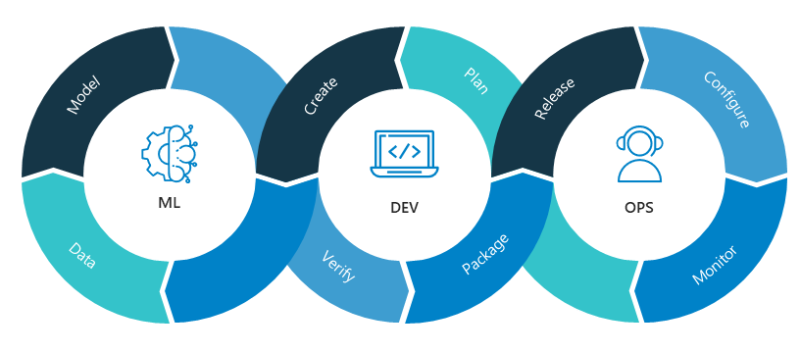
\includegraphics[width=0.5\textwidth]{./img/MLops/mlops.png}
      \caption{MLops}
      \label{fig:mlops}
\end{figure}
\begin{nota}
      Si parla solitamente di MLops quando ci si trova a gestire un numero elevato
      di pipeline. Questo permette di gestire in automatico tutte le pipeline e
      riuscire ad organizzare il lavoro in modo più efficiente.
\end{nota}

Uno strumento molto utile quando si parla di MLops sono i \textbf{feature store}.
Questi strumenti permettono di gestire in modo efficiente i processi di gestione
delle pipeline. In particolare, si ha una parte di \textbf{governance}, nella
quale sono memorizzati dei meta-dati che permettono di tenere traccia di tutte
le pipeline. Un esempio di questi meta-dati sono:
\begin{itemize}
      \item Le feature utilizzate.
      \item Il modello che è stato addestrato.
      \item Gli iperparametri utilizzati.
      \item etc\dots
\end{itemize}
\section{Data quality}
Rappresentare la realtà attraverso i dati è un processo molto complesso, perché
si utilizza un insieme finito di dati che approssimano la realta. Inoltre, tali
dati non sempre sono aggiornati e non sempre sono corretti.

Il problema è legato al fatto che le misure di qualità dei dati dipendono da
chi li utilizza e per cosa sono utilizzati. Solitamente si ha un trade off tra
utilità e realtà del dato.
\begin{definizione}[\textbf{Data Quality}]
      Non esiste una definizione precisa di data quality, ma possiamo dire che
      un dato è di buona qualità se è adatto all'uso che se ne vuole fare.
\end{definizione}

Quindi la qualità è una metrica soggettiva, possiamo però fornire una dimensione,
ovvero delle caratteristiche che descrivono la qualità dell'informazione.
Un esempio sono l'incompletezza, l'incorrettezza e l'inconsistenza.

Il problema di queste è che non sono misurabili. Quindi dovremo utilizzare delle
misure metriche, le quali vengono calcolate sui dati attraverso una specifica
procedura e hanno una unità di misura associata.

In generale abbiamo diverse metriche per ogni dato.

Le dimensioni sono tante ma si possono raggruppare nei seguenti gruppi:
\begin{itemize}
      \item Accuracy, Correctness, Precision
      \item Completeness, Pertinence
      \item Minimality, Redundancy, Compactness
      \item Consistency, Coherence
      \item Readability, Comprehensibility, Usability
      \item Accessibility, Usability
      \item Currency, Volatility, Timeliness
\end{itemize}
Oltre a questa divisione, le metriche possono essere divise tra:
\begin{itemize}
      \item Soggettive: misure di qualità che dipendono dalla percezione delle
            persone che  effettuano la misura.
      \item Oggettive: misure di qualità che non dipendono dalla percezione delle
            persone che effettuano la misura.
\end{itemize}
\subsection{Accuracy}
Una misura che possiamo fare oer verificare la qualità di un dato è l'accuracy.
Nello specifico, possiamo applicare questa metrica su dati alfanumerici,
tuple e relazioni.
\begin{definizione}[\textbf{Accuracy}]
      L'\textbf{accuracy} è una misura di qualità che esprime quanto un dato è
      vicino alla rappresentazione reale del fenomeno che si vuole rappresentare.
\end{definizione}
Dato che solitamente non conosciamo il valore reale del fenomeno, e che ottenerlo
potrebbe essere costoso, possiamo distinguere due tipologie di accuracy:
\begin{itemize}
      \item \textbf{Accuratezza semantica}: questa tipologia è definita quando si
            è a conoscenza dei valori reali, e misura quanto il dato si avvicina
            a questi valori.
      \item \textbf{Accuratezza sintattica}: è definito come il grado con il quale
            i dati rappresentano il mondo reale.
\end{itemize}
\begin{nota}
      Conoscere lo schema del dato pyò aiutare a valutare l'accuratezza.
\end{nota}
Come si può intuire dalle definizioni, risulta più difficile dimostrare l'accuratezza
semantica rispetto a quella sintattica.

Un modo per controllare l'accuratezza sintattica è quello di ottenere un elenco
di tutti valori del dominio dell'attributo e si cerca il valore a distanza minima.

Nel caso in cui si abbiano più valori, allora scegliamo quello più coerente col
record facendo dei controlli incrociati con altri attributi dello stesso record,
oppure è possibile inferire dalle frequenze dei valori dell'attributo degli altri
record.

Spesso non abbiamo un insieme completo di valori del dominio dell'attributo, quindi
è possibile utilizzare dagli altri valori degli attributi dello stesso record o
altri valori dello stesso attributo su record diverso.

Per controllare l'accuratezza di stringhe possiamo utilizzare la distanza di edit
normalizzata nel seguente modo:
\begin{equation*}
      1 - \frac{ED(x,y)}{n}
\end{equation*}
Abbiamo diverse tipologie di distanze che si applicano in base al formato del dato.
\subsection{Completeness}
Una misura di qualità che possiamo fare è la \textbf{completezza}. Essa specifica la
copertura con la quale il fenomeno osservato è rappresentato nell'insieme di dati.

Esistono diversi livelli di completezza, in particolare:
\begin{itemize}
      \item \textbf{Completezza di attributo}: misura il numero di valori nulli
            rispetto al numero di record.
      \item \textbf{Completezza di tupla}: misura il numero di valori nulli rispetto
            al numero di attributi.
      \item \textbf{Completezza di tabella}: misura il numero di valori nulli
            rispetto al numero di valori possibili.
      \item \textbf{Completezza di oggetto}: misura il numero di valori nulli
            rispetto al numero di valori possibili.
\end{itemize}
\subsection{Proprietà temporali}
Un'altra metrica di qualità è la \textbf{currency}, la quale misura la rapidita
di aggiornamento.Questa metrica è misurabile se c'è un file log degli arrivi e
degli aggiornamenti, oppure possiamo riferirci al metadato di ultimo aggiornamento.

Un'altra metrica è la \textbf{tempestività} che misura quanto i dati sono aggiornati
rispetto a un particolare processo (o ai processi) che li realizza.
\subsection{Consistenza}
Alla consistenza possono essere associati due significati:
\begin{itemize}
      \item Consistenza dei dati con i vincoli di integrità definiti sullo schema.
      \item Consistenza delle diverse rappresentazioni di uno stesso oggetto
            della realtà presenti nella base di dati.
\end{itemize}
I vincoli sulla consistenza si posso esprimere su gruppi di attributi, in particolare,
possiamo specificare:
\begin{itemize}
      \item Vincoli di integrità nel modello relazionale, come dipendenze funzionali
            o integrità referenziale.
      \item Vincoli di integrità in logica.
      \item Data edit nelle indagini statistiche.
\end{itemize}
\begin{nota}
      Non sempre si ha la possibilità di correggere un dato.
\end{nota}
\subsection{Accessibilità}
Esprime la capacità di un utente di accedere ai dati a partire dalla propria
cultura, stato fisico e psichico e della tecnologie disponibili.

In molti casi la bassa qualità dei dati dipende da diversi fattori. Una bassa
frequenza di aggiornamento può portare a una accuratezza minore del dato.

Il problema è che non possiamo avere massima qualità su qualsiasi metrica. Possiamo
pensare di avere massima accuratezza a discapito dell'aggiornamento temporale.

Esiste una fase di data improvement che serve a migliorare la qualità dei dati.
Questa fase può essere fatta seguendo due approcci:
\begin{itemize}
      \item \textbf{Data-driven}: si puliscono i dati una volta che sono stati
            raccolti. Questo approccio funziona bene quando si raccolgono i dati
            una volta sola.
      \item \textbf{Process-driven}: si puliscono i dati prima di integrarli.
            In questo approccio si puliscono i dati alla sorgente e non nel dataset.
            Per la realizzazione di questo approccio si possono seguire due metodi:
            \begin{itemize}
                  \item \textbf{Process drive}: vengono inseriti dei checkpoint
                        per controllare i dati che sono stati raccolti. Questo
                        viene fatto per evitare che i dati sporchi vengano integrati.
                  \item \textbf{Process redesign}: viene ridisegnato il processo
                        di raccolta dei dati per evitare che i dati sporchi vengano
                        integrati.
            \end{itemize}
\end{itemize}
\subsection{Data quality for ML}
I tipi di errori che si vogliono evitare:
\begin{itemize}
      \item \textbf{Noisy labels}: informazioni insufficienti date all'esperto,
            errori nell'etichetta, soggettività nell'etichettatura, problemi di
            comunicazione o codifica.

            Questi errori causano riduzione delle performance, possibili errori
            della feature selection\dots

            I possibili metodi per risolverli sono:
            \begin{itemize}
                  \item Scegliere algoritmi robusti rispetto la presenza di errori
                        nelle labels. Questi sono difficili da progettare e non
                        facilmente portabili e applicabili in altri contesti.
                  \item Approccio basato sui dati. Si eliminano le etichette sbagliate
                        e si costruisce un filtro per identificare eventuali errori
                        nelle labels, sfruttando SVM e CNN.
            \end{itemize}
      \item \textbf{Outliers}: causati da errori di data entry, misura strumento,
            sperimentali, campionamento, procedure nella fase di preprocessing, 
            oppure origine naturale.

            Gli algoritmi possono essere più o meno sensibili alla distribuzione. 
            Ad esempio, la regressione è sensibile agli outliers in base alla 
            loro posizione.
      \item \textbf{Overlapping data points}
      \item \textbf{Inconsistency}
      \item \textbf{Missing values}
\end{itemize}

L'ordine con cui si puliscono i dati cambia influenza l'efficacia dei metodi. 
Esistono diversi tool che possono essere usati per pulire i dati.